\documentclass[12pt,a4paper]{article}

% --- Packages ---
\usepackage{amsmath,amssymb}
\usepackage{booktabs}
\usepackage{graphicx}
\usepackage[hidelinks]{hyperref}
\usepackage{cleveref}
\usepackage[round,authoryear,sort&compress,longnamesfirst]{natbib}
\usepackage{geometry}
\usepackage{setspace}
\usepackage{enumitem}
\usepackage{url}
\usepackage{array}
\usepackage{tikz}
\usetikzlibrary{positioning,arrows.meta,decorations.pathreplacing,shapes.geometric,calc,backgrounds}

\geometry{margin=1in}
\setstretch{1.4}
\bibliographystyle{plainnat}

\begin{document}

% ============================================================
% COVER SHEET
% ============================================================
\thispagestyle{empty}
\begin{center}

\vspace*{2cm}

{\large\textbf{Qualifying Report}}

\vspace{2.5cm}

\begin{tabular}{r@{\hskip 6pt}l}
\textbf{Student Name (Student No.):} & Yiwei Gan (59765200) \\[8pt]
\textbf{Programme:} & Department of Data Science \\[8pt]
\textbf{Title of Research Proposal:} & \parbox[t]{9cm}{\raggedright\small Risk Behavior and Credit Signals in DeFi Lending Markets: Borrower Active Adjustment Under Position Risk Accumulation} \\[8pt]
\textbf{Report Type (Reporting Period):} & Qualifying Report (1 Aug 2025\,--\,31 Jul 2026) \\[8pt]
\textbf{Date:} & July 2026
\end{tabular}

\vfill
\rule{\textwidth}{0.5pt}
\footnotesize City University of Hong Kong \hspace{1cm} Department of Data Science

\end{center}

\newpage

% ============================================================
% TITLE PAGE (blind)
% ============================================================
\title{\vspace{-1.5cm} \textbf{Risk Behavior and Credit Signals in DeFi Lending Markets:}\\\large{Borrower Active Adjustment Under Position Risk Accumulation}}
\author{}
\date{}

\maketitle
\thispagestyle{empty}

\section*{Abstract}

Decentralized Finance (DeFi) has experienced exponential growth since 2020, with lending protocols such as Aave, Compound, and MakerDAO intermediating total value locked exceeding \$100 billion across multiple blockchain networks. These protocols operate entirely through smart contracts that govern collateralization, borrowing, and liquidation automatically, creating a fully transparent on-chain record of all participant behavior. However, the academic literature on DeFi lending has predominantly focused on protocol-level risk exposure, liquidation mechanics, and aggregate market efficiency, devoting considerably less attention to the micro-level behavioral responses of individual borrowers as their positions approach risky thresholds. This research report surveys the relevant literature across three interconnected domains—DeFi lending infrastructure, behavioral finance and prospect theory, and on-chain credit risk assessment—and identifies a specific, underexplored research gap at their intersection. We propose a study that investigates whether borrowers' active adjustments during periods of rising position risk provide risk information beyond that captured by conventional on-chain indicators such as health factor, collateralization ratio, and account activity. The proposed methodology reconstructs position-risk trajectories from publicly available blockchain data, classifies borrower-initiated actions separately from passive liquidation events, and tests the incremental predictive contribution of behavioral process variables using a discrimination framework. A discussion of possible outcomes, including contributions to DeFi protocol design and credit risk modeling, as well as a critical assessment of the study's boundaries, is provided.

\vspace{8pt}
\noindent\textbf{Keywords:} Decentralized Finance, DeFi lending, behavioral finance, prospect theory, credit risk, blockchain analytics, on-chain data

\newpage
\tableofcontents
\newpage

\section{Introduction}

The emergence of decentralized finance represents one of the most significant structural transformations in financial intermediation since the advent of electronic trading. Between January 2020 and December 2025, the total value locked (TVL) in DeFi protocols expanded from under \$1 billion to over \$100 billion at its peak, with lending protocols consistently accounting for the largest share of this activity~\cite{schar2021decentralized2, jiang2023defi}. Unlike traditional financial intermediaries, which rely on institutional credit assessment, relationship-based lending, and regulatory compliance frameworks to manage risk, DeFi lending protocols operate through immutable smart contracts that algorithmically enforce collateralization requirements, interest rate adjustments, and automatic liquidation of under-collateralized positions~\cite{gudgeon2020defi}. The complete transparency of these protocols means that every deposit, withdrawal, borrowing event, repayment, collateral adjustment, and liquidation is immutably recorded on a public blockchain, creating an unprecedented empirical window into the behavior of financial market participants operating under varying degrees of risk exposure.

This transparency has given rise to a rapidly growing literature that examines DeFi lending from multiple analytical angles. One strand of research investigates the systemic risks inherent in these protocols, including liquidity crunches, cascading liquidations, and the potential for contagion across composable DeFi primitives~\cite{qin2021empirical, perez2020liquidations}. A second strand develops risk modeling frameworks tailored to the unique features of DeFi lending, including multi-chain environments, cross-protocol dependencies, and institutional-grade risk taxonomies~\cite{oberholzer2026toward, sevim2026interoperability}. A third strand applies machine learning methods to on-chain data for credit scoring and default prediction~\cite{ghosh2024onchain}. A fourth strand examines the engineering properties of specific protocol mechanisms, including liquidation thresholds, interest rate curves, and governance design~\cite{iftikhar2025automated, tovanich2023contagion}. 

Despite the richness of this literature, a notable gap persists at its core. The existing research on DeFi lending risk has focused overwhelmingly on what might be termed \emph{state variables}—static snapshots of position health captured by health factors, collateralization ratios, and borrowing volumes at discrete time points. What has received considerably less empirical attention is the \emph{behavioral process} through which borrowers navigate rising position risk: the active decisions they make to adjust collateral, repay debt, increase their exposure, or maintain their positions as their risk profile deteriorates. This distinction matters because two borrowers with identical health factors at a given moment may follow fundamentally different trajectories depending on their behavioral responses to mounting risk pressure. One borrower may proactively add collateral and reduce leverage early in the risk cycle, while another may maintain or even increase exposure until forced into liquidation by third-party arbitrageurs. Conventional risk indicators would place these two borrowers at the same level of risk, yet their behavioral processes suggest meaningfully different approaches to risk management that may contain information about future outcomes.

This research report addresses this gap by proposing a study situated at the intersection of DeFi lending infrastructure, behavioral finance theory, and on-chain credit risk assessment. The central research question we propose is: In public on-chain lending markets, do borrowers' active adjustments under rising position risk provide risk information beyond that contained in conventional on-chain indicators? This question decomposes into two analytically distinct but empirically connected layers. The first, behavioral layer asks whether borrowers exhibit systematic patterns of active adjustment as their positions approach risky thresholds—patterns that are distinguishable from random or purely mechanical responses to price movements. The second, credit-oriented layer asks whether these behavioral patterns, if they exist, carry incremental predictive power for future liquidation events or risk deterioration beyond what is already captured by health factors, collateral ratios, and account activity measures.

%
% Figure 1: Conceptual Framework
%
\begin{figure}[t]
\centering
\resizebox{\textwidth}{!}{%
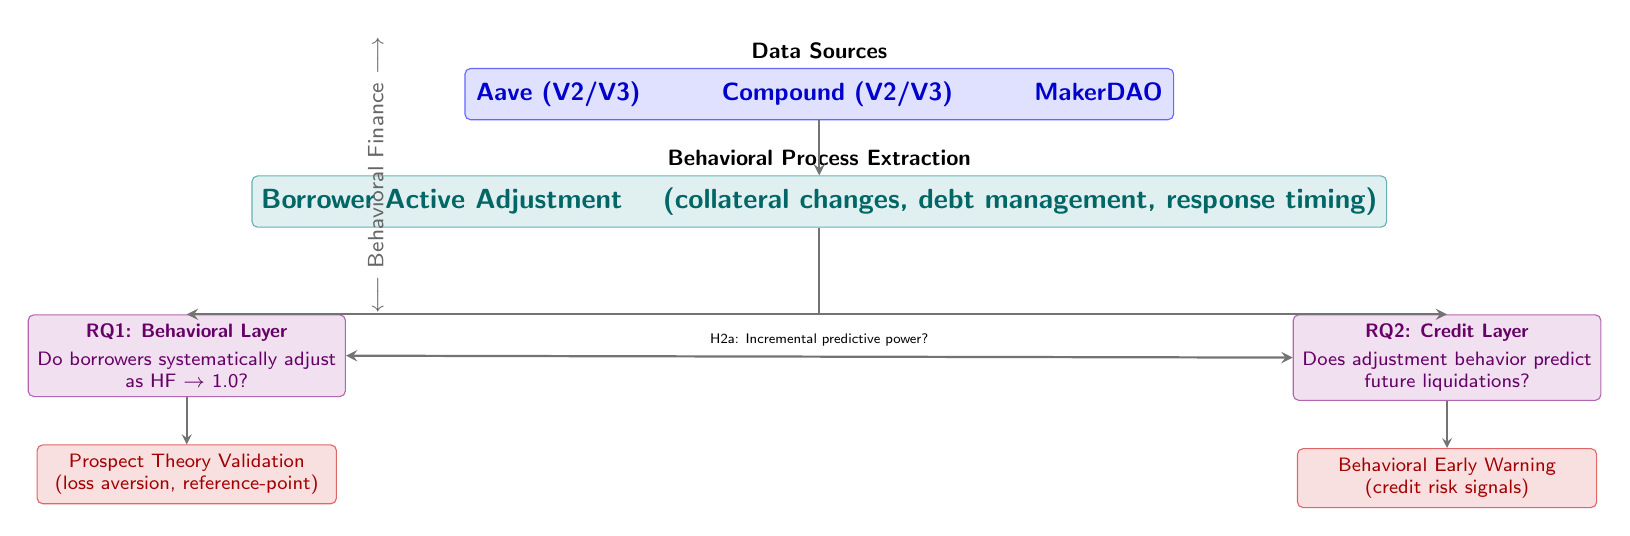
\begin{tikzpicture}[
  node distance=1.2cm and 0.6cm,
  box/.style={rectangle, rounded corners=2pt, draw=#1!60, fill=#1!12, text=#1!80!black, minimum width=2.2cm, minimum height=0.65cm, align=center, font=\scriptsize\sffamily, line width=0.4pt},
  widebox/.style={rectangle, rounded corners=2pt, draw=#1!60, fill=#1!12, text=#1!80!black, minimum width=9cm, minimum height=0.65cm, align=center, font=\small\sffamily\bfseries, line width=0.4pt},
  smallbox/.style={rectangle, rounded corners=2pt, draw=#1!60, fill=#1!10, text=#1!80!black, minimum width=1.8cm, minimum height=0.5cm, align=center, font=\tiny\sffamily, line width=0.3pt},
  arrow/.style={->, >=stealth, line width=0.6pt, draw=black!55},
  darrow/.style={<->, >=stealth, line width=0.7pt, draw=black!55},
]
  % Layer 1: Protocols
  \node[widebox=blue, label={[font=\footnotesize\sffamily\bfseries]north:Data Sources}] (proto) {Aave (V2/V3) \hspace{0.8cm} Compound (V2/V3) \hspace{0.8cm} MakerDAO};

  % Layer 2: Behavioral variables  
  \node[widebox=teal, below=0.7cm of proto, label={[font=\footnotesize\sffamily\bfseries]north:Behavioral Process Extraction}] (behave) {\normalsize Borrower Active Adjustment \quad (collateral changes, debt management, response timing)};

  % Layer 3: Two tracks
  \node[box=violet, below left=1.1cm and -1.2cm of behave, minimum width=3.8cm, font=\scriptsize\sffamily] (rq1) {\textbf{RQ1: Behavioral Layer}\\[2pt]Do borrowers systematically adjust\\as HF $\rightarrow$ 1.0?};
  \node[box=violet, below right=1.1cm and -1.2cm of behave, minimum width=3.8cm, font=\scriptsize\sffamily] (rq2) {\textbf{RQ2: Credit Layer}\\[2pt]Does adjustment behavior predict\\future liquidations?};

  \node[box=red!80!black, below=0.6cm of rq1, minimum width=3.8cm, font=\scriptsize\sffamily] (out1) {Prospect Theory Validation\\(loss aversion, reference-point)};
  \node[box=red!80!black, below=0.6cm of rq2, minimum width=3.8cm, font=\scriptsize\sffamily] (out2) {Behavioral Early Warning\\(credit risk signals)};

  % Arrows
  \draw[arrow, thick] (proto.south) -- (behave.north);
  \draw[arrow, thick] (behave.south) |- (rq1.north);
  \draw[arrow, thick] (behave.south) |- (rq2.north);
  \draw[arrow] (rq1.south) -- (out1.north);
  \draw[arrow] (rq2.south) -- (out2.north);
  \draw[darrow, thick] (rq1.east) -- node[above, font=\tiny\sffamily]{H2a: Incremental predictive power?} (rq2.west);

  % Left labels
  \node[font=\footnotesize\sffamily, text=black!60, rotate=90, above left=0.0cm and -1.8cm of behave, anchor=south] {$\longleftarrow$ Behavioral Finance $\longrightarrow$};
\end{tikzpicture}%
}
\caption{Conceptual framework for studying borrower behavior and credit signals in DeFi lending. The framework proceeds from raw on-chain data (top) through behavioral process variable extraction (center) to the research questions (bottom). RQ1 characterizes how borrowers adjust positions as risk accumulates; RQ2 tests whether these behavioral patterns provide incremental predictive power for future liquidation events beyond conventional risk indicators.}
\label{fig:framework}
\end{figure}

\vspace{4pt}

The report is organized as follows. Section~2 surveys the relevant literature across three domains: DeFi lending infrastructure and risk, behavioral finance and prospect theory, and on-chain credit risk assessment. Section~3 identifies the specific research topic and articulates the research questions and hypotheses. Section~4 describes the proposed research methodology, including data sources, variable construction, and analytical framework. Section~5 discusses possible outcomes, contributions, limitations, and boundary conditions.

\newpage
\section{Literature Review}

The proposed research sits at the intersection of three distinct but interconnected bodies of scholarly literature: (1) the architecture, risk, and empirical study of DeFi lending protocols, (2) behavioral finance theory, with particular emphasis on prospect theory as a framework for understanding decision-making under risk, and (3) the emerging literature on on-chain credit risk assessment and the use of blockchain data for predictive modeling of financial outcomes. This section reviews each of these domains in turn, identifying both their individual contributions and the specific gap that motivates the proposed study.

\subsection{DeFi Lending: Architecture, Risks, and Empirical Evidence}

DeFi lending protocols represent the most capital-intensive and empirically scrutinized segment of the decentralized finance ecosystem. These protocols enable permissionless borrowing and lending of crypto-assets through smart contracts that algorithmically manage collateralization, interest rates, and liquidation events without relying on traditional financial intermediaries~\cite{schar2021decentralized2}. The fundamental mechanism is straightforward: a borrower deposits crypto-assets as collateral and may borrow another asset up to a fraction of the collateral's value, defined by the protocol's loan-to-value (LTV) parameter. If the value of the collateral declines relative to the borrowed amount—or if the value of the borrowed asset increases—the position's health factor (HF) deteriorates. Once the HF falls below the liquidation threshold (typically 1.0), any network participant can trigger a liquidation, repaying part of the debt and claiming the corresponding collateral plus a liquidation bonus~\cite{perez2020liquidations, qin2021empirical}.

The academic literature examining these mechanisms from an empirical perspective has grown considerably. \citet{perez2020liquidations} provided one of the earliest systematic analyses of liquidation events across DeFi lending platforms, documenting that liquidations occur frequently, involve substantial transaction fees, and can create cascading risk when multiple protocols are involved. \citet{qin2021empirical} extended this analysis by examining the incentive structures created by liquidation bonuses and demonstrating how these incentives can lead to competitive ``priority gas auctions'' among liquidators during periods of high market volatility. \citet{sun2022liquidity} analyzed liquidity risk in Aave, showing that large borrowing positions can create substantial utilization pressure in specific asset pools, potentially limiting the ability of smaller depositors to withdraw.

More recently, a growing body of work has focused on cross-protocol risk and the systemic dimensions of DeFi lending. \citet{tovanich2023contagion} studied financial contagion in Compound V2, constructing protocol balance sheets and demonstrating how concentrated borrowing positions can create non-trivial default risk that propagates through interconnected liquidity pools. \citet{sevim2026interoperability} extended risk modeling to multi-chain environments, showing that cross-chain interoperability introduces new categories of risk that are not captured by single-chain models. \citet{oberholzer2026toward} proposed a comprehensive nine-dimension risk assessment framework for institutional DeFi, encompassing counterparty, market, liquidity, operational, governance, legal, regulatory, smart contract, and oracle risks. \citet{iftikhar2025automated} conducted a cross-chain comparative analysis of automated risk management mechanisms in Aave and Compound, highlighting important differences in how these two dominant lending protocols handle parameter adjustments and liquidation execution.

A recurring characteristic of this literature is its focus on the protocol-level or system-level perspective. Whether analyzing liquidation cascades, interest rate dynamics, or cross-protocol dependencies, the unit of analysis is typically the protocol, the liquidity pool, or the set of interacting smart contracts. The individual borrower—as a decision-making agent whose behavior may vary systematically with risk exposure—enters the analysis primarily as a source of demand for protocol services rather than as an object of study in its own right. Understanding how borrowers actively navigate risk accumulation and whether their behavioral responses carry credit-relevant information therefore constitutes a complementary analytical perspective that the existing protocol-centric literature has not yet systematically explored.

\subsection{Prospect Theory and Financial Decision-Making Under Risk}

Since its original formulation by \citet{kahneman1979prospect} and its subsequent extension to Cumulative Prospect Theory by \citet{tversky1992advances}, prospect theory (PT) has become one of the most influential frameworks in behavioral economics for understanding how individuals make decisions under conditions of risk and uncertainty. The theory identifies several systematic deviations from the predictions of expected utility theory. First, individuals evaluate outcomes relative to a reference point, typically the status quo, rather than in terms of final wealth levels. Second, their value function is concave in the domain of gains (risk aversion) and convex in the domain of losses (loss aversion), with the disutility of losses being approximately twice as large as the utility of equivalent gains. Third, individuals exhibit diminishing sensitivity, meaning that the marginal impact of an outcome decreases as one moves farther from the reference point. Fourth, decision weights are systematically non-linear in objective probabilities, with low-probability events being overweighted and moderate-to-high-probability events being underweighted.

These theoretical predictions have received extensive empirical support across a wide range of financial domains. \citet{benartzi1995myopic} demonstrated that myopic loss aversion—the combination of loss aversion with frequent portfolio evaluation—can explain the equity premium puzzle, one of the most prominent anomalies in financial economics. \citet{barberis2013thirty}, in a comprehensive review, documented that prospect theory has been successfully applied to explain the disposition effect in stock trading, the pricing of initial public offerings, the equity premium, and a range of other financial market phenomena. The theory has become a cornerstone of behavioral finance, providing a parsimonious framework that rationalizes empirical regularities that are difficult to explain within the standard rational expectations paradigm.

However, the application of prospect theory to DeFi lending markets presents both opportunities and challenges. On the one hand, DeFi lending provides an almost ideal empirical laboratory for testing behavioral theories. The liquidation threshold—a hard-coded, protocol-defined health factor value below which positions become eligible for liquidation—serves as an objective, exogenously determined reference point that is identical across all participants. This stands in contrast to traditional financial settings, where reference points are typically unobserved, subjective, and likely to vary across individuals~\cite{barberis2013thirty}. Furthermore, the complete observability of all borrower actions in DeFi—including collateral additions, debt repayment, additional borrowing, and collateral withdrawals—means that behavioral responses to proximity to the liquidation threshold can be measured with a level of granularity that would be impossible in traditional credit markets.

On the other hand, there are significant challenges to applying prospect theory in this context. DeFi borrowers may not perceive the protocol-defined liquidation threshold as their psychological reference point; they may instead anchor on their initial entry price, a portfolio-level target return, or other benchmarks. Moreover, the rational incentive to avoid liquidation—which imposes a non-trivial financial penalty in the form of the liquidation bonus paid to the liquidator—provides a powerful non-behavioral explanation for active position management near the liquidation threshold. Disentangling rational risk management from behavioral deviations therefore requires careful empirical design, including the use of control groups, instrumental variables, or regression discontinuity approaches that exploit the quasi-exogenous variation created by the protocol-defined liquidation threshold.

\subsection{On-Chain Credit Risk Assessment}

The third body of literature relevant to this proposal concerns the use of on-chain data for credit risk assessment and default prediction. The fundamental premise of this emerging field is that the transparency of blockchain data makes it possible to construct credit risk models without relying on the centralized credit bureaus, bank account information, or traditional financial records that underpin conventional credit scoring systems.

Several recent studies have demonstrated the feasibility of this approach. \citet{ghosh2024onchain} developed a framework for on-chain credit risk scoring in DeFi, using machine learning models trained on wallet-level transaction histories, borrowing and repayment patterns, and interaction frequencies to predict the likelihood of default. Their results suggest that on-chain behavioral data contains significant credit-relevant information, even in the absence of off-chain identity information. \citet{xu2021banks} traced the evolution of lending markets from traditional banking to decentralized finance, arguing that DeFi protocols can potentially improve capital efficiency by enabling more granular and transparent risk assessment. Various survey papers have consolidated the range of DeFi risk factors that can be extracted from on-chain data, including transaction graphs, holding patterns, and interaction histories across multiple protocols~\cite{werner2022sok, jiang2023defi}.

However, the existing on-chain credit risk literature has important limitations that the current proposal seeks to address. First, the majority of studies treat credit risk as a static classification problem: given a set of features observed at time \(t\), predict whether the borrower will default at time \(t+k\). While this approach has produced useful results, it does not capture the \emph{dynamics} of how borrowers actively manage their positions as risk accumulates. A borrower who experiences a gradual decline in their health factor over several weeks and responds by systematically adding collateral and reducing leverage may face a fundamentally different risk profile than a borrower with an identical point-in-time health factor who has experienced the same decline without any adjustment activity—yet static models would assign them identical risk scores.

Second, the existing literature has focused primarily on relatively broad on-chain activity measures—such as total transaction count, account age, interaction diversity, and protocol-level aggregates—rather than on the specific behavioral processes that occur as positions approach risky thresholds. The theoretical distinction between state variables (what the position looks like at a point in time) and process variables (how the position evolved to its current state and how the borrower responded during that evolution) has not been systematically incorporated into empirical credit risk models, despite its prominence in the broader financial economics literature on the informational content of trading behavior.

\subsection{Identifying the Gap}

The preceding review identifies a clear gap at the intersection of these three bodies of literature. DeFi lending research has thoroughly documented the mechanisms of liquidation, contagion, and systemic risk from a protocol perspective but has not systematically examined borrower behavior as a source of credit signals. Behavioral finance, encapsulated by prospect theory, provides a rich theoretical framework for understanding how individuals respond to losses and reference points but has seen only limited application to DeFi lending contexts. The on-chain credit risk literature has demonstrated that blockchain data can support predictive models of borrower default but has employed predominantly static and feature-based approaches that do not capture the processual nature of borrower risk management.

The gap, stated explicitly, is: \emph{There is no systematic empirical study that examines whether borrowers' active adjustments during periods of rising position risk in DeFi lending markets contain risk information beyond that captured by conventional on-chain state variables, and whether the behavioral patterns observed are consistent with the predictions of prospect theory.}

This gap is worth addressing for both academic and practical reasons. Academically, testing whether behavioral process variables carry incremental predictive power would connect two largely separate research traditions—the protocol-centric analysis of DeFi risk and the individual-centric tradition of behavioral finance—that have the potential to inform and enrich each other. Practically, demonstrating that active borrower behavior contains independent risk signals would have immediate implications for protocol design, including the potential to complement existing risk parameters with behaviorally-informed early warning indicators.

\newpage

\section{Identification of the Research Topic}

\subsection{Research Context and Motivation}

The preceding literature review identifies a specific, underexplored research question that sits at the intersection of DeFi lending risk, behavioral finance, and on-chain credit assessment. This section articulates the specific research topic that the proposed study seeks to address, including its scope, its research questions, and the falsifiable hypotheses that would guide empirical testing.

The proposed research is motivated by the following observation: DeFi lending protocols generate a comprehensive, time-stamped record of every action taken by every participant, yet the existing literature has predominantly treated these data as a source of static features for cross-sectional risk classification rather than as a window into the dynamic process through which borrowers manage, or fail to manage, mounting risk exposure. This is a missed opportunity because the temporal dimension of borrower behavior—the sequence, timing, and magnitude of active adjustments relative to changes in position health—may contain credit-relevant information that is not captured by point-in-time snapshots of collateralization ratios, health factors, or other conventional risk indicators.

The research topic is therefore defined as follows: \textbf{The empirical relationship between borrowers' active behavioral adjustments in response to rising position risk in DeFi lending protocols and the subsequent likelihood of liquidation or other adverse risk outcomes.} This topic is situated within the broader domain of financial risk assessment but distinguishes itself through its emphasis on behavioral process variables rather than state variables, its use of publicly verifiable on-chain data, and its grounding in the theoretical frameworks of behavioral finance.

\subsection{Research Questions}

The proposed study addresses two hierarchically organized research questions:

\begin{description}[leftmargin=*,labelindent=\parindent, itemindent=0pt]
\item[RQ1 (Behavioral Layer).] When a DeFi borrower's position approaches the protocol-defined liquidation threshold, do borrowers exhibit systematic, non-random patterns of active adjustment—in the form of collateral additions, debt repayment, position closure, or continued risk-taking—that are distinguishable from the mechanical effects of price movements and liquidation bot activity?

\item[RQ2 (Credit Layer).] Controlling for conventional on-chain risk indicators, including current health factor, collateral ratio, account activity, asset concentration, and market volatility, do behavioral process variables capturing the \emph{trajectory} of active adjustments provide statistically and economically significant incremental predictive power for future liquidation events?
\end{description}

RQ1 asks whether there is a behavioral phenomenon worth explaining: a question about the existence, magnitude, and structure of active borrower responses to risk accumulation. This question is primarily descriptive and has value in its own right, even in the absence of credit prediction results. RQ2 asks whether that phenomenon has practical relevance for risk assessment: a question about the added value of behavioral information beyond what is already available from simpler, more direct risk indicators. The hierarchical structure of the research questions means that RQ2 is conditional on RQ1: if there is no systematic behavioral response to position risk, the question of whether such responses predict outcomes is moot.

\subsection{Hypotheses}

The research questions translate into the following falsifiable hypotheses:

\subsubsection*{RQ1: Behavioral Hypotheses}

\begin{description}[leftmargin=*,labelindent=\parindent, itemindent=0pt]
\item[H1a (Active Adjustment Occurrence).] The probability of observing a borrower-initiated collateral addition or debt repayment increases monotonically as the health factor approaches the liquidation threshold from above, after controlling for contemporaneous price movements of the underlying collateral assets.

\item[H1b (Loss Aversion Asymmetry).] The magnitude of borrower-initiated risk-reducing actions (collateral additions, debt repayment) per unit deterioration in health factor is larger in absolute value than the magnitude of additional borrowing or collateral withdrawal per unit improvement in health factor, consistent with the loss aversion prediction of prospect theory.

\item[H1c (Reference-Point Discontinuity).] There is a discontinuity in the probability of observing active risk-reducing behavior at the health factor value corresponding to the liquidation threshold, above and beyond the smooth relationship that would be predicted by a model using only collateral price movements.
\end{description}

\subsubsection*{RQ2: Credit Prediction Hypotheses}

\begin{description}[leftmargin=*,labelindent=\parindent, itemindent=0pt]
\item[H2a (Incremental Predictive Power).] A model that includes behavioral process variables—specifically, the presence, timing, and magnitude of active adjustments made as the position approaches the liquidation threshold—achieves significantly better out-of-sample prediction of liquidation events than a model using only conventional on-chain risk indicators.

\item[H2b (Temporal Precedence).] Behavioral adjustment variables measured in period \(t-1\) to \(t\) improve the prediction of liquidation events in period \(t\) to \(t+k\) even after controlling for the health factor and its recent trajectory up to time \(t\).
\end{description}

\subsection{Positioning and Novelty}

The proposed study contributes to the existing literature in three distinct ways. First, it shifts the analytical focus of DeFi lending research from protocol-level risk to borrower-level behavior, introducing a micro-foundation for understanding how the participants in DeFi markets respond to the incentive structures created by smart contract parameters. Second, it bridges the largely separate literatures on DeFi risk modeling and behavioral finance by testing prospect theory predictions in a naturalistic financial setting where the reference point—the liquidation threshold—is objective, observable, and identical for all participants, thereby addressing a key measurement challenge that has limited the external validity of many behavioral finance studies~\cite{barberis2013thirty}. Third, it introduces a process-based perspective on credit risk assessment that complements the static, feature-based approaches that have dominated the on-chain credit risk literature to date~\cite{ghosh2024onchain}, potentially opening new avenues for the construction of behavioral early warning indicators in DeFi lending protocols.

It is important to be precise about what this study does \emph{not} claim. It does not claim that DeFi borrowers are irrational or that their behavior necessarily deviates from the predictions of rational expectations models. The empirical approach is designed to test whether behavioral variables \emph{add information} beyond conventional risk indicators, not to adjudicate between competing models of rationality. It does not claim that behavioral process variables are better predictors of liquidation than conventional indicators; the hypotheses are framed explicitly in terms of \emph{incremental} predictive power rather than absolute accuracy. And it does not claim that any observed behavioral patterns necessarily generalize to other DeFi protocols, time periods, or market conditions; external validity is a matter for subsequent replication and extension.

%
% Figure 3: Risk Trajectory / Health Factor Illustration
%
\begin{figure}[t]
\centering
\resizebox{\textwidth}{!}{%
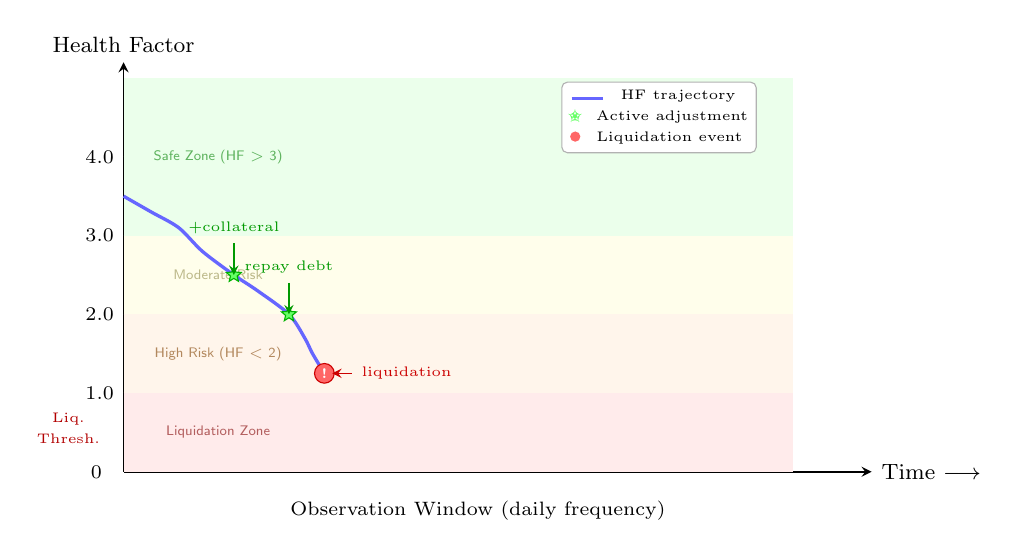
\begin{tikzpicture}[
  scale=1.0,
  >=stealth,
  axisline/.style={->, line width=0.6pt},
  dataline/.style={line width=0.8pt},
]
  % Axes
  \draw[axisline] (0,0) -- (9.5,0) node[right, font=\footnotesize] {Time $\longrightarrow$};
  \draw[axisline] (0,0) -- (0,5.2) node[above, font=\footnotesize] {Health Factor};
  
  % Labels
  \node[font=\scriptsize] at (4.5,-0.5) {Observation Window (daily frequency)};
  
  % Y-axis labels
  \draw[dashed, gray!40] (0,0.0) -- (8.5,0.0);
  \node[font=\scriptsize, left] at (-0.15,0.0) {0};
  \draw[dashed, gray!40] (0,1.0) -- (8.5,1.0);
  \node[font=\scriptsize, left] at (0,1.0) {1.0};
  \node[font=\tiny, red!70!black] at (-0.7, 0.55) {\shortstack{Liq.\\Thresh.}};
  
  \draw[dashed, gray!40] (0,2.0) -- (8.5,2.0);
  \node[font=\scriptsize, left] at (0,2.0) {2.0};
  \draw[dashed, gray!40] (0,3.0) -- (8.5,3.0);
  \node[font=\scriptsize, left] at (0,3.0) {3.0};
  \draw[dashed, gray!40] (0,4.0) -- (8.5,4.0);
  \node[font=\scriptsize, left] at (0,4.0) {4.0};
  
  % Risk bands (shaded)
  \fill[red!8] (0,1.0) rectangle (8.5,0.0);
  \fill[orange!8] (0,2.0) rectangle (8.5,1.0);
  \fill[yellow!8] (0,3.0) rectangle (8.5,2.0);
  \fill[green!8] (0,5.0) rectangle (8.5,3.0);
  
  \node[font=\tiny\sffamily, text=red!50!black, opacity=0.6] at (1.2,0.5) {Liquidation Zone};
  \node[font=\tiny\sffamily, text=orange!50!black, opacity=0.6] at (1.2,1.5) {High Risk (HF $<$ 2)};
  \node[font=\tiny\sffamily, text=yellow!50!black, opacity=0.6] at (1.2,2.5) {Moderate Risk};
  \node[font=\tiny\sffamily, text=green!50!black, opacity=0.6] at (1.2,4.0) {Safe Zone (HF $>$ 3)};
  
  % Simulated HF trajectory
  \draw[dataline, blue!60, line width=1.2pt] plot[smooth] coordinates {
    (0,3.5) (0.35,3.3) (0.7,3.1) (1.0,2.8) (1.4,2.5) (1.7,2.3) 
    (2.1,2.0) (2.3,1.7) (2.4,1.5) (2.55,1.25) 
  };
  
  % Active adjustment events (stars)
  \node[star, star points=5, star point ratio=2.25, draw=green!70!black, fill=green!60, minimum size=2mm, inner sep=0pt] at (1.4,2.5) {};
  \draw[->, green!60!black, line width=0.5pt] (1.4,2.9) -- (1.4,2.5) node[pos=0, above, font=\tiny] {+collateral};
  
  \node[star, star points=5, star point ratio=2.25, draw=green!70!black, fill=green!60, minimum size=2mm, inner sep=0pt] at (2.1,2.0) {};
  \draw[->, green!60!black, line width=0.5pt] (2.1,2.4) -- (2.1,2.0) node[pos=0, above, font=\tiny] {repay debt};
  
  % Liquidation event
  \node[circle, draw=red!80!black, fill=red!60, minimum size=2.5mm, inner sep=0pt] at (2.55,1.25) {\tiny\color{white}\textbf{!}};
  \draw[->, red!80!black, line width=0.5pt] (2.9,1.25) -- (2.65,1.25) node[pos=0, right, font=\tiny] {liquidation};
  
  % Legend (inside plot area, top right)
  \node[font=\tiny, draw=black!30, fill=white, rounded corners=2pt, inner sep=3pt] at (6.8,4.5) {
    \shortstack[l]{
      \tikz{\draw[blue!60, line width=1.1pt] (0,0)--(0.4,0);} \, HF trajectory\\
      \tikz{\node[star, star points=5, star point ratio=2.25, fill=green!60, minimum size=1.3mm, inner sep=0pt] at (0,0) {};} \, Active adjustment\\
      \tikz{\node[circle, fill=red!60, minimum size=1.3mm, inner sep=0pt] at (0,0) {};} \, Liquidation event
    }
  };

\end{tikzpicture}%
}
\caption{Illustrative health factor (HF) trajectory and behavioral response. A borrowing position's HF declines toward the liquidation threshold (HF = 1.0) as collateral value decreases. Active borrower adjustments (green stars) represent collateral additions or debt repayment. The central empirical question is whether the pattern of these adjustments—their timing, magnitude, and frequency—provides predictive information about eventual liquidation beyond what is captured by the HF itself.}
\label{fig:trajectory}
\end{figure}

\vspace{4pt}

\newpage
\section{Research Methodology}

This section describes the proposed research design, including the data sources, sample construction, variable operationalization, and analytical strategy. The methodology is designed to test the falsifiable hypotheses specified in Section~3 within a framework that maximizes internal validity while acknowledging the inherent limitations of observational data from permissionless financial protocols.

\subsection{Data Sources and Protocol Selection}

The proposed study relies exclusively on publicly available on-chain data from Ethereum-based DeFi lending protocols. This choice of data sources is deliberate and relates to an important feature of the research design: because all transactions on the Ethereum blockchain are publicly visible and verifiable, the study can be independently replicated by any researcher with access to blockchain infrastructure, without depending on proprietary datasets, platform partnerships, or commercial data licensing agreements.

The primary data source will be the historical event logs and state data from three major DeFi lending protocols: Aave (V2 and V3), Compound (V2 and V3), and MakerDAO. These three protocols collectively account for the majority of DeFi lending activity on Ethereum and offer complementary data for cross-protocol validation. The specific event types to be extracted include: (i) \texttt{Deposit} and \texttt{Withdraw} events, representing the provision and removal of collateral; (ii) \texttt{Borrow} and \texttt{Repay} events, representing the creation and settlement of loan positions; (iii) \texttt{LiquidationCall} or equivalent events, capturing the triggering of liquidation by third parties; and (iv) \texttt{FlashLoan} events for identifying transactions that may involve complex multi-step strategies rather than simple borrowing behavior.

Data will be extracted using Dune Analytics, a community-maintained blockchain data platform that provides SQL-queryable access to decoded event logs and state data. Price data for the underlying collateral assets will be obtained from on-chain price oracles (Chainlink) to ensure that the price information used in the analysis matches the price information actually available to protocol participants at the time of each event. The study period will span from the genesis of each protocol through the most recent complete month of data availability at the time of analysis, ensuring coverage of multiple market cycles and varying levels of DeFi ecosystem activity.

\subsection{Unit of Analysis and Sample Construction}

The primary unit of analysis is the \textbf{borrower-position-month}—that is, a specific borrowing position held by a specific wallet address during a given calendar month. This choice of analytical unit is motivated by several considerations. First, it allows the study to track the evolution of individual positions over time, capturing the dynamic process of risk accumulation and borrower response that is central to the research questions. Second, it accommodates the fact that a single wallet address may hold multiple independent borrowing positions within and across protocols, and allows the analysis to control for within-address correlation of errors using clustered standard errors at the wallet level. Third, it aligns with the temporal frequency at which most DeFi risk metrics are conventionally reported and consumed.

The sample will include all borrowing positions for which the following criteria are met: (i) the borrowing event occurred during or after the protocol's deployment on Ethereum mainnet and before the data extraction date; (ii) the borrowing position had a non-zero health factor at some point during the observation window; and (iii) the position involved one of the major borrowing assets supported by the protocol (ETH, WBTC, USDC, USDT, DAI). Positions that are exclusively part of leveraged yield farming strategies, identifiable by circular borrowing patterns involving the same asset, will be flagged and analyzed separately to assess robustness.

\subsection{Active vs.\ Passive Classification}

A critical element of the methodology is the operational distinction between active, borrower-initiated actions and passive, externally-driven events. This distinction is essential because the research question concerns borrower behavior, and conflating active borrower decisions with events triggered by third parties or protocol mechanics would severely undermine the validity of the analysis.

The classification will proceed as follows. An on-chain transaction will be classified as an \textbf{active borrower action} if and only if the transaction sender (\texttt{msg.sender}) matches the borrower wallet address. Under this criterion, the following events will be classified as active: (i) depositing additional collateral, (ii) repaying an outstanding loan, (iii) withdrawing collateral (when permitted by the protocol), (iv) borrowing additional assets, and (v) closing a position by fully repaying the outstanding debt and withdrawing all collateral. A transaction will be classified as a \textbf{passive liquidation event} if the transaction sender is an address other than the borrower, regardless of whether that address can be identified as a known liquidation bot.

This classification rule has the important advantage of being fully deterministic and replicable: any researcher with access to the raw transaction data can apply it identically. Its primary limitation is that it cannot distinguish between cases where the borrower is the initiator of the transaction (true active behavior) and cases where the borrower delegates transaction signing to a third-party service, although the analysis can include robustness checks that restrict the sample to addresses where the majority of transactions are self-initiated based on transaction nonce patterns.

\subsection{Position Risk Trajectory Reconstruction}

For each borrowing position, a trajectory of position health will be reconstructed at a daily frequency. The core risk metric is the \textbf{health factor} (HF), defined as:

\begin{equation}
\text{HF}_t = \frac{\sum_{i} (C_{i,t} \cdot P_{i,t}) \cdot \text{LTV}_i}{D_t}
\end{equation}

where \(C_{i,t}\) is the quantity of collateral asset \(i\) at time \(t\), \(P_{i,t}\) is its price, \(\text{LTV}_i\) is the protocol-specific loan-to-value parameter for that asset, and \(D_t\) is the total outstanding debt denominated in a common currency unit. The HF equals 1.0 at the liquidation threshold, with lower values indicating higher risk.

The trajectory reconstruction will also compute a set of derived variables that characterize the temporal evolution of the position: (i) the minimum health factor attained over the trailing 7, 14, and 30 days; (ii) the number of days the position spent in various health factor bands (e.g., below 1.2, 1.2--1.5, 1.5--2.0, above 2.0); (iii) the maximum drawdown in health factor over the trailing 30 days; and (iv) the time elapsed since the position entered its current health factor band.

\subsection{Behavioral Process Variables}

The explanatory variables of primary interest capture the borrower's active behavioral response to changes in position risk. The following variables will be constructed for each borrower-position-month:

\begin{description}[leftmargin=*,labelindent=\parindent, itemindent=0pt]
\item[Active Collateral Adjustment Rate.] The net amount of collateral added or withdrawn by the borrower during the observation month, scaled by the average total collateral value over the same period. Positive values indicate net addition of collateral (risk-reducing) and negative values indicate net withdrawal (risk-increasing).

\item[Active Debt Management Rate.] The net amount of debt repaid or newly borrowed during the observation month, scaled by the average total debt over the same period. Positive values indicate net borrowing and negative values indicate net repayment.

\item[Response Latency.] The number of days between the date on which the health factor first crossed below a given threshold (e.g., 1.5, 1.3, 1.1) and the date of the borrower's first subsequent active collateral addition or debt repayment. Long latencies indicate passive behavior in the face of rising risk.

\item[Adjustment Intensity.] The absolute magnitude of collateral added or debt repaid at the first adjustment following entry into a new risk band, expressed as a proportion of the total position value. This captures whether the borrower made a small, tentative adjustment or a large, decisive one.

\item[Behavioral Consistency.] A measure of how closely the borrower's behavior over time conforms to a rule-based adjustment policy. Borrowers who add collateral predictably as their health factor declines will receive high consistency scores; those whose behavior appears random or reactive to price movements rather than risk will receive low scores.
\end{description}

\subsection{Control Variables}

To isolate the incremental contribution of behavioral process variables, models will include a comprehensive set of control variables drawn from four domains:

\begin{enumerate}[leftmargin=*,labelindent=\parindent, itemindent=0pt]
\item \textbf{Current risk state:} The point-in-time health factor, collateral ratio, and the proportion of total collateral held in volatile assets.
\item \textbf{Account characteristics:} The wallet's age, total number of past transactions across all DeFi protocols, number of distinct protocols interacted with, and total value of historical borrowing.
\item \textbf{Asset composition:} Dummy variables for the specific assets used as collateral and borrowed, and a Herfindahl-Hirschman Index (HHI) of asset concentration within the position.
\item \textbf{Market conditions:} The trailing 30-day annualized volatility of the collateral asset, the correlation between collateral and borrowed asset prices, and dummy variables for periods of elevated gas costs that might inhibit active position management.
\end{enumerate}

\subsection{Analytical Framework}

The analysis will proceed in three stages, corresponding to the hierarchical structure of the research questions.

%
% Figure 2: Methodology Pipeline
%
\begin{figure}[t]
\centering
\resizebox{\textwidth}{!}{%
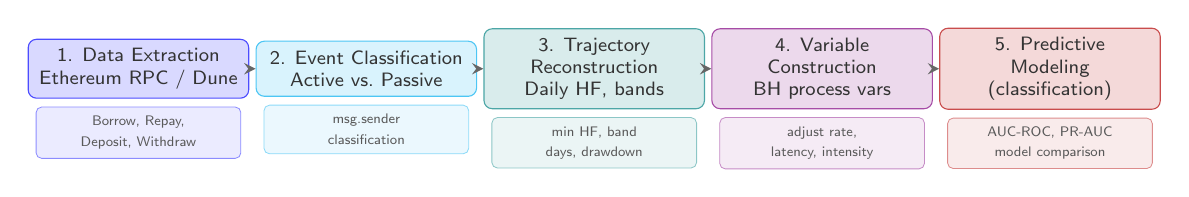
\begin{tikzpicture}[
  node distance=0.7cm and 0.4cm,
  stage/.style={rectangle, rounded corners=3pt, draw=#1!70, fill=#1!15, text=black!80, minimum width=2.8cm, minimum height=0.7cm, align=center, font=\scriptsize\sffamily, line width=0.4pt},
  substage/.style={rectangle, rounded corners=2pt, draw=#1!45, fill=#1!8, text=black!65, minimum width=2.6cm, minimum height=0.5cm, align=center, font=\tiny\sffamily, line width=0.3pt},
  arrow/.style={->, >=stealth, line width=0.6pt, draw=black!60},
]
  \node[stage=blue] (s1) {1. Data Extraction\\Ethereum RPC / Dune};
  \node[stage=cyan, right=0.08cm of s1] (s2) {2. Event Classification\\Active vs.\ Passive};
  \node[stage=teal, right=0.08cm of s2] (s3) {3. Trajectory\\Reconstruction\\Daily HF, bands};
  \node[stage=violet, right=0.08cm of s3] (s4) {4. Variable\\Construction\\BH process vars};
  \node[stage=red!70!black, right=0.08cm of s4] (s5) {5. Predictive\\Modeling\\(classification)};

  \draw[arrow, thick] (s1.east) -- (s2.west);
  \draw[arrow, thick] (s2.east) -- (s3.west);
  \draw[arrow, thick] (s3.east) -- (s4.west);
  \draw[arrow, thick] (s4.east) -- (s5.west);

  \node[substage=blue, below=0.1cm of s1] {\shortstack{Borrow, Repay,\\Deposit, Withdraw}};
  \node[substage=cyan, below=0.1cm of s2] {\shortstack{msg.sender\\classification}};
  \node[substage=teal, below=0.1cm of s3] {\shortstack{min HF, band\\days, drawdown}};
  \node[substage=violet, below=0.1cm of s4] {\shortstack{adjust rate,\\latency, intensity}};
  \node[substage=red!70!black, below=0.1cm of s5] {\shortstack{AUC-ROC, PR-AUC\\model comparison}};
\end{tikzpicture}%
}
\caption{Methodology pipeline from raw blockchain data to predictive model evaluation. Stage 1 extracts transaction events from Ethereum; Stage 2 classifies transactions as active (borrower-initiated) or passive (liquidation bot); Stage 3 reconstructs position risk trajectories; Stage 4 constructs behavioral process variables; and Stage 5 estimates predictive models using standard classification techniques, evaluating them $\rightarrow$ liquidation prediction at 7d/30d/90d horizons.}
\label{fig:methodology}
\end{figure}

\vspace{4pt}

\paragraph{Stage 1: Behavioral Description (RQ1).} The objective of this stage is to characterize the empirical relationship between position health and active borrower behavior. The primary analytical tool is the estimation of the following panel regression model:

\begin{equation}
\text{Action}_{i,t} = \alpha + \beta_1 \text{HF}_{i,t-1} + \beta_2 \text{HF}_{i,t-1}^2 + \gamma_1 \Delta P_{i,t} + \delta \mathbf{X}_{i,t-1} + \eta_i + \tau_t + \varepsilon_{i,t}
\end{equation}

where \(\text{Action}_{i,t}\) is a measure of active borrower behavior (collateral addition, debt repayment), \(\text{HF}_{i,t-1}\) is the lagged health factor, \(\Delta P_{i,t}\) are contemporaneous price changes, \(\mathbf{X}_{i,t-1}\) is a vector of time-varying controls, \(\eta_i\) captures time-invariant borrower-specific heterogeneity through fixed effects, and \(\tau_t\) captures common time effects. H1a is tested through the sign and significance of \(\beta_1\), which should be negative if borrowers respond to declining health factors (i.e., increasing risk) by taking risk-reducing actions. H1b is tested by comparing the coefficient on health factor declines (loss domain) to the coefficient on health factor increases (gain domain) on the absolute value of borrowing actions. H1c is tested by augmenting the model with an indicator variable for the position being within a narrow band around the liquidation threshold and interacting this indicator with the health factor.

\paragraph{Stage 2: Predictive Framework (RQ2).} The objective of this stage is to test whether behavioral process variables contain incremental predictive power for liquidation events. The analytical framework for this stage is a model comparison, or ``horse race,'' in which progressively richer sets of predictor variables are compared on their ability to predict liquidation events in a held-out test sample. The following models will be estimated:

\begin{itemize}[leftmargin=*,labelindent=\parindent, itemindent=0pt]
\item \textbf{M0 (Baseline):} A logistic regression model using only the current health factor, collateral ratio, and the interaction between them.
\item \textbf{M1 (State Variables):} M0 augmented with the set of risk state, account characteristic, and asset composition variables described in Section~4.5.
\item \textbf{M2 (State + Market Variables):} M1 augmented with market condition variables, including collateral asset volatility and gas price indicators.
\item \textbf{M3 (Full Model):} M2 augmented with the behavioral process variables described in Section~4.4.
\end{itemize}

All models will be estimated using gradient-boosted decision trees (XGBoost) rather than logistic regression as the primary specification, with the logistic regression results reported as robustness checks. The choice of tree-based models is motivated by their ability to capture non-linear relationships and complex interactions among predictor variables without requiring explicit specification by the researcher, which is important given the absence of strong theoretical priors about the functional form of the predictive relationships.

Model performance will be evaluated using standard classification metrics—area under the receiver operating characteristic curve (AUC-ROC), precision-recall AUC, and calibration error—computed on a temporally separated hold-out test set using a rolling window evaluation scheme that simulates realistic out-of-sample conditions. Statistical significance of differences in AUC between models will be assessed using DeLong's test. H2a will be supported if M3 achieves significantly higher AUC than M2. It is important to note the stringency of this test: because M3 contains all the variables in M2 plus the behavioral process variables, any observed improvement in predictive performance is directly attributable to the information content of the behavioral variables and cannot be attributed to the inclusion of additional variables per se.

\paragraph{Stage 3: Robustness.} A series of robustness checks will assess the sensitivity of the results to specific methodological choices. These will include: (i) re-estimating all models using logistic regression and comparing results between the tree-based and linear specifications; (ii) varying the prediction horizon (7-day, 30-day, and 90-day ahead liquidation prediction); (iii) restricting the sample to borrowers who have interacted with the protocol for at least a minimum number of days to exclude very new users; (iv) repeating the analysis separately for each protocol to assess cross-protocol generalizability; and (v) conducting a variable importance decomposition to quantify the relative contribution of state variables, market variables, and behavioral process variables to the overall predictive performance of the full model.

\newpage
\section{Discussion and Possible Outcomes}

This section discusses the range of possible outcomes from the proposed study, their implications for the academic literature and for DeFi protocol design, and the boundary conditions that constrain the interpretation and generalizability of the results. Unlike studies that present a single hypothesized outcome, this discussion acknowledges that the results could take several forms, each with distinct implications.

\subsection{Scenario 1: Behavioral Process Variables Matter (H2a Supported)}

The most favorable outcome from the perspective of the study's theoretical contribution is that behavioral process variables contain statistically significant and economically meaningful incremental predictive power for liquidation events, above and beyond conventional on-chain risk indicators. If this scenario materializes, the results would indicate that \emph{how} a borrower's position arrived at its current state—the sequence of active adjustments, the timing of responses to risk signals, and the consistency of risk management behavior—carries information about future outcomes that is not fully captured by what the position's current state happens to be. This finding would be consistent with a growing body of evidence in financial economics suggesting that the process of portfolio management, not merely the resulting portfolio composition, contains information about investor sophistication and future performance.

The contribution of such a finding would be threefold. First, at the theoretical level, it would provide the first systematic evidence that prospect theory's predictions—particularly those concerning loss aversion and reference-point effects—are observable in DeFi lending behavior at a granular, position-by-position level. The unique features of the DeFi setting—objective, protocol-defined reference points; complete behavioral observability; and the absence of confounding factors associated with traditional financial intermediation—would make this evidence particularly compelling from a research design perspective and would contribute to the broader program of testing behavioral finance theories in naturalistic settings.

Second, at the empirical level, it would introduce a new category of predictor variables—behavioral process variables—to the on-chain credit risk toolkit. While the incremental predictive power of these variables might be modest in absolute terms (as is typically the case when building on a strong baseline model), even a small but statistically significant improvement in predictive power could be practically relevant in the context of DeFi protocols, where even marginal improvements in liquidation prediction can have substantial economic consequences given the volumes involved.

Third, at the practical level, the results would suggest that DeFi protocols could complement their existing, purely state-dependent risk assessment mechanisms with behavioral early-warning indicators. For example, a protocol might monitor the rate at which borrowers in a specific health factor band are actively adjusting their positions, treating an abnormally low rate of adjustment among risky positions as an aggregate signal of forthcoming liquidation pressure.

\subsection{Scenario 2: Behavior is Systematic but Not Predictive (RQ1 Supported; RQ2 Not Supported)}

An alternative possible outcome is that the behavioral hypotheses of RQ1 are supported—borrowers do exhibit systematic patterns of active adjustment as their positions approach risky thresholds, and these patterns are consistent with the predictions of prospect theory—but that RQ2 is not supported because behavioral process variables do not provide statistically significant incremental predictive power beyond conventional risk indicators. In this scenario, the findings would demonstrate that borrower behavior near the liquidation threshold is structured rather than random, and that this structure can be described using the theoretical framework of prospect theory, but that the information contained in this behavioral structure is already fully captured by simpler, more direct risk indicators. The health factor itself, possibly supplemented by its recent trajectory and the current market volatility environment, might be a sufficient statistic for the credit-relevant information contained in borrower behavior.

While this scenario would fall short of the study's more ambitious contribution, it would nonetheless represent a valuable addition to the literature. It would provide what is, to the best of our knowledge, the first systematic empirical characterization of how DeFi borrowers actively manage—or fail to manage—their positions as risk accumulates. This empirical contribution would be valuable even in the absence of predictive success, as it would document a set of stylized facts about borrower behavior that could inform future theoretical and empirical work.

\subsection{Scenario 3: No Systematic Behavior or Predictive Power (RQ1 and RQ2 Not Supported)}

The least favorable outcome from the perspective of publication prospects is that neither RQ1 nor RQ2 is supported: borrowers do not exhibit systematic patterns of active adjustment as their positions approach the liquidation threshold, and behavioral process variables do not improve predictions of liquidation events. In this scenario, the data would suggest that DeFi borrowers' behavior near the liquidation threshold is either random, driven entirely by the mechanical effects of price movements and liquidation bot activity, or dominated by factors that the study is unable to observe.

Even in this scenario, the study would have produced a useful null result. The transparency of DeFi protocols means that the research design and data are fully replicable, and the hypotheses are falsifiable and were specified ex ante. However, a null result in this setting is more likely to reflect genuine absence of an effect than other frequently-invoked explanations for non-replication in the social sciences, such as researcher degrees of freedom or publication bias. Indeed, one plausible interpretation of this outcome is that DeFi lending markets are relatively efficient, with borrowers responding to the strong financial incentives created by liquidation penalties in a manner that is well-approximated by standard risk measures. This interpretation would itself be a finding of interest to researchers studying the efficiency of DeFi markets relative to traditional financial markets, where behavioral biases are more consistently documented.

\subsection{Contributions and Implications}

The proposed study has the potential to make contributions at multiple levels. At the methodological level, it would demonstrate a template for how publicly available blockchain data can be used to conduct detailed, process-oriented behavioral research without relying on proprietary datasets or platform partnerships. At the theoretical level, it would provide a systematic test of behavioral finance predictions in a novel empirical setting that offers unusually clean identification of the relevant theoretical constructs. At the practical level, it would inform the design of DeFi protocols by evaluating whether borrower behavior contains credit-relevant information that could complement existing, state-based risk assessment mechanisms.

The implications of the study extend beyond the specific context of DeFi lending. The broader question addressed—whether the \emph{process} of risk management contains information beyond the \emph{state} of risk exposure—applies to a wide range of financial contexts, from margin trading in traditional securities markets to the management of corporate debt structures. Demonstrating that this question can be answered in the affirmative using DeFi data would provide a proof of concept for a research program that could eventually extend to these other contexts, where the necessary data would be considerably more difficult to obtain.

\subsection{Limitations and Boundary Conditions}

The proposed study has several important limitations that constrain the interpretation and generalizability of its results, regardless of which of the three scenarios described above materializes.

\textbf{Partial observability of user behavior.} The analysis is limited to on-chain transactions, which means that it cannot observe borrower behavior on centralized exchanges or off-chain activities. A borrower who appears to be relatively passive on-chain may be actively hedging their position on a centralized exchange, and a borrower who appears to be actively adjusting their position on-chain may be doing so for reasons unrelated to the risk of that specific position. This partial observability is an inherent limitation of research using public blockchain data and should be explicitly acknowledged rather than minimized.

\textbf{Cannot infer intent from on-chain data.} While the classification of transactions as active borrower actions or passive liquidations is straightforward and replicable, the motives underlying those actions cannot be observed. A borrower who adds collateral following a decline in their health factor may be responding to the risk of liquidation, but they could also be responding to factors that are correlated with—but conceptually distinct from—position risk, such as a change in their assessment of the collateral asset's future price trajectory or a desire to maintain a specific portfolio allocation.

\textbf{Limited external validity.} The study is focused on a specific set of DeFi lending protocols during a specific period of market development. The extent to which the findings would generalize to other protocols, other time periods, or other types of blockchain-based financial applications is unknown and would need to be evaluated through replication and extension. The rapid pace of change in the DeFi ecosystem—including ongoing changes to protocol parameters, the introduction of new lending mechanisms, and the evolution of the competitive landscape—means that even findings that are internally valid at the time of analysis may have a limited shelf life.

\textbf{Confounding by unobserved borrower characteristics.} While panel data methods with borrower fixed effects will be used to control for time-invariant unobserved heterogeneity, it remains possible that time-varying unobserved factors—such as changes in a borrower's financial circumstances, risk preferences, or access to alternative sources of liquidity—could influence both their behavioral responses to risk accumulation and their subsequent likelihood of liquidation, creating a spurious association between behavioral process variables and liquidation outcomes. The observational nature of the data means that the study can identify associations but cannot establish causal relationships.

\subsection{Ethical Considerations}

The proposed research uses only publicly available on-chain data that does not contain personally identifiable information. No individual user will be contacted or re-identified from their wallet address, and the analysis will be conducted exclusively at the level of aggregates and statistical summaries. Nevertheless, the study touches on broader ethical questions about the use of public blockchain data for credit assessment. Following the work of this study, protocols might seek to incorporate behavioral variables into risk assessment, and this could have consequences for borrowers that are not easily anticipated. It is worth noting that the relationship between active position adjustment and credit outcomes is assessed at the aggregate level; the estimates cannot be meaningfully interpreted as individual-level predictions without careful attention to issues of statistical discrimination and fairness.

\subsection{Future Research Directions}

The proposed study opens several avenues for future research, some of which can be anticipated at this stage and others that will become apparent only after the empirical results are available. First, if the behavioral process variables are found to have incremental predictive power, subsequent research could investigate the mechanisms underlying this relationship using more detailed decomposition analyses or structural estimation. Second, the framework developed in this study could be extended to other DeFi lending protocols operating on different blockchain networks, providing evidence on the generalizability of the results across different protocol designs and market environments. Third, research could investigate the welfare implications of incorporating behavioral process variables into protocol risk parameters, considering both the potential benefits of improved risk assessment and the potential costs associated with increased protocol complexity. Fourth, future work could examine whether borrowers who exhibit systematic patterns of active position management in DeFi have different characteristics or outcomes in traditional credit markets, conditional on the availability of data that links the two domains.

\newpage

\bibliography{refs_参考文献}

\end{document}
